\documentclass[11pt]{article}

% ---------------------------------------------------------------------------
% Packages
% ---------------------------------------------------------------------------
\usepackage[utf8]{inputenc}
\usepackage[T1]{fontenc}
\usepackage[a4paper,margin=1in]{geometry}
\usepackage{amsmath,amssymb}
\usepackage{booktabs}
\usepackage{graphicx}
\usepackage{xcolor}
\usepackage{listings}
\usepackage{tikz}
\usepackage{pgfplots}
\pgfplotsset{compat=1.17}
\usepackage[colorlinks=true,linkcolor=blue,citecolor=blue,urlcolor=blue]{hyperref}

% ---------------------------------------------------------------------------
% Listings style (blue keywords, green comments, red strings)
% ---------------------------------------------------------------------------
\definecolor{codekw}{RGB}{0,0,180}
\definecolor{codecomment}{RGB}{0,128,0}
\definecolor{codestring}{RGB}{163,21,21}
\definecolor{codebg}{RGB}{245,245,245}
\lstdefinestyle{py}{
  language=Python,
  basicstyle=\ttfamily\footnotesize,
  keywordstyle=\color{codekw}\bfseries,
  commentstyle=\color{codecomment}\itshape,
  stringstyle=\color{codestring},
  numbers=left,
  numberstyle=\tiny\color{gray},
  backgroundcolor=\color{codebg},
  frame=single,
  rulecolor=\color{gray!40},
  breaklines=true,
  showstringspaces=false,
  columns=fullflexible,
}
\lstdefinestyle{sh}{
  language=bash,
  basicstyle=\ttfamily\footnotesize,
  keywordstyle=\color{codekw},
  commentstyle=\color{codecomment}\itshape,
  stringstyle=\color{codestring},
  numbers=left,
  numberstyle=\tiny\color{gray},
  backgroundcolor=\color{codebg},
  frame=single,
  rulecolor=\color{gray!40},
  breaklines=true,
  showstringspaces=false,
  columns=fullflexible,
}

\title{\vspace{-1.5em}\textbf{Detecting Hallucinations in Large Language Models via the
vLLM-Hook Framework}\\[0.4em]
\large Porting an H-Node Probe Detector to the Post-Refactor vLLM-Hook Plugin Architecture}
\author{Samarpit Bhatia\\
Indian Institute of Technology, Bombay\\
\texttt{24b0603@iitb.ac.in}}
\date{June 2026}

\begin{document}
\maketitle

% ---------------------------------------------------------------------------
\begin{abstract}
This report documents the \emph{migration and re-validation} of a hallucination-detection
pipeline onto the current release of IBM's \textbf{vLLM-Hook} framework. An earlier version
of this work implemented Phase~1 (the \emph{detection} stage) of the H-Node Adversarial
Neural Computation framework of Yocam et al.\ (2026) against an older vLLM-Hook revision,
on \texttt{Qwen2.5-3B-Instruct}. Since then, upstream has substantially rewritten the plugin
core: per-request configuration moved from process environment variables to
\texttt{SamplingParams.extra\_args}; the worker is installed through
\texttt{worker\_extension\_cls} rather than \texttt{worker\_cls}; a new general-plugin
(\texttt{\_hook\_plugin}) captures probe artifacts via \texttt{collective\_rpc}; and the
analyzer contract changed to \texttt{analyze(spec, run\_id, probes)}. We rebase our feature
cleanly onto upstream, adapt the \texttt{HallucinationAnalyzer} to the new contract, and
switch activation capture to the framework's deterministic disk path. Re-validated on a
single consumer laptop (NVIDIA RTX~4060, 8\,GB VRAM) with \texttt{Qwen2.5-1.5B-Instruct} and
600 TruthfulQA prompts, the trained probe attains a held-out ROC--AUC of \textbf{0.902} at
layer~14 of~28 ($\sim$50\% depth), reproducing the characteristic mid-network AUC peak. The
complete three-stage \emph{extract--train--detect} pipeline runs end-to-end on the new
framework, confirming that the detection use case survives the upstream rewrite without any
modification to the framework core. We additionally report the non-trivial dependency- and
environment-engineering required to bring up the new stack on the target machine.
\end{abstract}

\tableofcontents
\bigskip

% ===========================================================================
\section{Introduction}

\subsection{Problem statement}
Large Language Models (LLMs) exhibit a well-documented failure mode known as
\emph{hallucination}: the generation of text that is fluent and confident but factually
incorrect or unsupported by the input. As LLMs are deployed in high-stakes applications, the
ability to flag a generation as potentially hallucinated --- ideally at inference time and
with low overhead --- has become central to safe deployment. Mechanistic-interpretability
work suggests that the propensity to hallucinate is encoded in a small number of
\emph{hidden-state dimensions} concentrated in the middle-to-late transformer blocks. If
true, this enables a lightweight white-box detector: train a linear probe on mid-layer hidden
states and, at inference time, score each prompt by reading those same activations off the
live forward pass.

\subsection{Context: from an older fork to the current framework}
The earlier iteration of this project was built and tuned against an older vLLM-Hook revision
and, after a hardware migration, finalised on \texttt{Qwen2.5-3B-Instruct} running under
\texttt{vllm==0.7.3}. Several of those commits were workarounds specific to that
configuration (e.g.\ forcing the \texttt{TRITON\_ATTN}/\texttt{XFORMERS} attention backend on
a compute-capability~7.5 GPU, and pinning \texttt{transformers==4.49.0}). In the interim,
upstream \texttt{IBM/vLLM-Hook} merged a major framework rewrite (the ``Spotlight'' attention
steering feature alongside a re-architected plugin core). The starting artefact for the work
reported here is therefore the \emph{rebased} repository: our detection feature re-applied on
top of the latest upstream commit, adapted to the new plugin contracts.

\subsection{The post-refactor vLLM-Hook framework}
vLLM-Hook\footnote{\url{https://github.com/IBM/vLLM-Hook}} augments
vLLM~\cite{vllm} with the ability to install PyTorch \texttt{forward\_hooks} on arbitrary
transformer modules \emph{without} modifying vLLM's core. The current release exposes:
\begin{itemize}
  \item A \emph{worker extension} (\texttt{ProbeHiddenStatesWorker}) installed via vLLM's
  \texttt{worker\_extension\_cls}. During the forward pass it captures last-token hidden
  states and, depending on the request's \texttt{extra\_args}, either returns them in-memory
  (RPC) or flushes them to a per-run artifact on shared memory / disk.
  \item A new general-plugin, \texttt{\_hook\_plugin}, registered through vLLM's
  \texttt{vllm.general\_plugins} entry-point group. It patches \texttt{LLM.generate} /
  \texttt{AsyncLLM.generate} to install the hooks and to retrieve captured probes through
  \texttt{collective\_rpc}, attaching them to the request output as \texttt{output.probes}.
  \item A \texttt{HookLLM} offline wrapper and a \texttt{HookClient} (for \texttt{vllm serve})
  that expose \texttt{.generate()} / \texttt{.analyze()}, configured per request through
  \texttt{SamplingParams.extra\_args} (offline) or \texttt{vllm\_xargs} (serve) --- no longer
  through environment variables.
  \item A registry-based plugin system: analyzer/worker pairs are added without touching the
  framework core, via \texttt{PluginRegistry.register\_analyzer / register\_worker}.
\end{itemize}

\subsection{Research question and scope}
The task can be stated as a single hypothesis:
\begin{quote}\itshape
Does the H-Node detection use case survive the upstream framework rewrite --- can the
detector be re-expressed entirely within the new plugin contracts, with no changes to the
framework core, and does it still produce a usable signal on commodity hardware?
\end{quote}
We answer in the affirmative. We:
\begin{enumerate}
  \item Rebase the feature onto the latest upstream and adapt \texttt{HallucinationAnalyzer}
  to the new \texttt{analyze(spec, run\_id, probes)} contract, sourcing hidden states through
  the framework's \texttt{unpack\_hidden\_states} / \texttt{load\_and\_merge\_hs\_cache}
  helpers.
  \item Construct a labelled dataset of 600 prompts from TruthfulQA~\cite{truthfulqa} and use
  it to train per-layer logistic-regression probes on the hidden states of
  \texttt{Qwen/Qwen2.5-1.5B-Instruct}.
  \item Demonstrate end-to-end detection on novel prompts at inference time on an 8\,GB
  laptop GPU, and document the dependency/environment engineering required to do so.
\end{enumerate}

% ===========================================================================
\section{Background: The H-Node Framework}

The H-Node Adversarial Neural Computation (ANC) framework of Yocam et al.~\cite{hnode} is a
three-phase methodology for studying hallucinations in LLMs:
\begin{description}
  \item[Phase 1 --- Detection.] Train a linear probe on each transformer layer's last-token
  hidden state, identify the layer with the highest predictive AUC, and extract the top-$N$
  hidden-state dimensions (the \emph{H-Nodes}) whose values most strongly drive the probe's
  hallucination prediction.
  \item[Phase 2 --- Attack.] Perturb the H-Nodes at inference time to \emph{induce}
  hallucinations in otherwise-grounded generations.
  \item[Phase 3 --- Defense.] Apply gradient-based ANC corrections to the same H-Nodes to
  suppress hallucinated outputs.
\end{description}
This project scopes itself strictly to Phase~1. The attack and defense phases require writing
modifications back into the residual stream, which would necessitate a steering worker; they
are left as future work (Section~\ref{sec:future}).

\subsection{Mathematical formulation}
Let $h_t^{(\ell)} \in \mathbb{R}^d$ denote the last-token hidden state at transformer layer
$\ell \in \{1,\dots,L\}$ for prompt $t$. Given a training set
$\mathcal{D} = \{(h_t^{(\ell)}, y_t)\}_{t=1}^{N}$ where $y_t \in \{0,1\}$ labels each prompt
as grounded (0) or hallucinated (1), we fit an $\ell_2$-regularised logistic regression at
each layer:
\begin{equation}
\hat{y}_t = \sigma\!\left(\mathbf{w}^{(\ell)\top} h_t^{(\ell)} + b^{(\ell)}\right),
\qquad \sigma(z) = \frac{1}{1+e^{-z}}.
\end{equation}
The \emph{best layer} $\ell^\star$ is the one with the highest held-out ROC--AUC:
\begin{equation}
\ell^\star = \arg\max_\ell \ \mathrm{AUC}\!\left(\mathbf{w}^{(\ell)}, b^{(\ell)};
\mathcal{D}_{\mathrm{eval}}\right).
\end{equation}
The H-Node set $\mathcal{H} \subset \{1,\dots,d\}$ is the top-$N$ dimensions of
$\mathbf{w}^{(\ell^\star)}$ by positive coefficient:
\begin{equation}
\mathcal{H} = \text{top-}N\!\left(\mathbf{w}^{(\ell^\star)}\right).
\end{equation}
A per-node \emph{grounded baseline} $b_j$ is the $80^{\text{th}}$-percentile activation among
grounded training samples, for each $j \in \mathcal{H}$. At inference time the \emph{H-Node
excess} of a new prompt $t'$ is
\begin{equation}
e_{t'} = \frac{1}{|\mathcal{H}|} \sum_{j \in \mathcal{H}}
\max\!\left(0,\ h_{t',j}^{(\ell^\star)} - b_j\right).
\end{equation}
The pair $(\hat{y}_{t'}, e_{t'})$ together provide a probabilistic verdict and a mechanistic
explanation: the probability is calibrated for classification, while the excess identifies
\emph{which} hallucination direction was activated.

% ===========================================================================
\section{Methodology}

The implementation factors into three CLI-invokable stages, each run as an independent
process: \texttt{python examples/demo\_halludetect.py [extract|train|detect]}. Only the
extract and detect stages require a GPU.

\subsection{Dataset construction}
We use the multiple-choice split (MC1) of TruthfulQA~\cite{truthfulqa}. For each of 300
randomly-sampled questions we generate two prompts:
\begin{itemize}
  \item One \emph{grounded} prompt of the form \texttt{Q: \{q\} \textbackslash n A: \{c\}}
  where $c$ is a randomly-sampled \emph{correct} answer from the MC1 labels.
  \item One \emph{hallucinated} prompt with $c$ replaced by a randomly-sampled
  \emph{incorrect} answer.
\end{itemize}
This yields a balanced set of 600 prompts (300 grounded / 300 hallucinated). A bare
\texttt{Q:/A:} format is used rather than a chat template, to keep the activation-space signal
as clean as possible. To prevent train/test leakage at the question level, we apply a
\emph{question-grouped} split (\texttt{train\_frac}=0.7), yielding 420 training and 180
held-out prompts.

\subsection{Activation extraction (\texttt{extract})}
This stage instantiates \texttt{HookLLM} with \texttt{worker\_name="probe\_hidden\_states"},
\texttt{analyzer\_name="hidden\_states"}, and a model-specific JSON config listing every
transformer layer ($1,\dots,28$ for Qwen2.5-1.5B-Instruct).

For each batch of prompts we issue a single-token generation (only the prefill activations are
needed). Crucially, we use the framework's \emph{disk path}: each batch is generated with
\texttt{save\_to\_disk=True} and a unique \texttt{run\_id}, which causes the worker to flush
the whole batch into one merged artifact; the main process then reads it back through
\texttt{llm.analyze(run\_id=...)} (the \texttt{HiddenStatesAnalyzer} with
\texttt{reduce="none"}). We adopt the disk path rather than the per-request in-memory
\texttt{output.probes} path because the latter only attaches probes to a request whose own
capture is non-empty, and is therefore not reliable for multi-prompt batches
(Section~\ref{sec:challenges}). Per-layer tensors are accumulated in prompt order; the final
artefact is a single \texttt{activations.pt} bundle
\[
\{\, \texttt{layer\_num} \mapsto \text{tensor of shape } (N,d) \,\}_{1 \le \texttt{layer\_num} \le 28}
\]
plus a label vector and question-ID list (the latter lets the train stage reproduce the same
question-grouped split).

\subsection{Probe training (\texttt{train})}
Pure CPU. For each layer we $z$-score normalise the activations using a
\texttt{StandardScaler} fit on the training rows only, then fit an $\ell_2$-regularised
\texttt{LogisticRegression} ($C{=}1.0$, lbfgs, 2000 iters, fixed seed). The held-out AUC is
computed on the eval rows, and the best layer $\ell^\star$ is selected by $\arg\max$. We then
extract the top $N{=}50$ H-Node indices by positive coefficient and compute the per-node
grounded baseline as the $80^{\text{th}}$ percentile of grounded-training-row activations. The
full artefact (\texttt{probe.npz} + \texttt{probe.json} metadata sidecar) stores
$\mathbf{w}^{(\ell^\star)}$, $b^{(\ell^\star)}$, the scaler statistics, $\mathcal{H}$, the
per-node baselines, and the full per-layer AUC dictionary. The script then rewrites the
inference config JSON, replacing the \texttt{layers} field with $[\ell^\star]$ so that the
\texttt{detect} stage installs hooks on only the single layer the probe needs.

\subsection{Live detection (\texttt{detect})}
This stage instantiates \texttt{HookLLM} with the narrow inference config and the registered
\texttt{analyzer\_name="hallucination"}. Each prompt batch is generated with
\texttt{save\_to\_disk=True} and a \texttt{run\_id}; the following
\texttt{llm.analyze(analyzer\_spec=\{"probe\_path": ...\}, run\_id=...)} call routes to the
\texttt{HallucinationAnalyzer}, which loads the probe, reads the best-layer hidden states from
the run artifact, and returns a result dictionary with per-prompt probability, H-Node excess,
raw margin, and verdict.

% ===========================================================================
\section{Implementation}

\subsection{Files}
All feature code lives in two locations: a top-level \texttt{hallucination\_detection/}
package containing model-agnostic training and scoring logic, and a single analyzer file
inside the framework's \texttt{vllm\_hook\_plugins/} package directory. Table~\ref{tab:files}
lists the artefacts.

\begin{table}[h]
\centering
\caption{Feature files re-applied on top of upstream. LOC counts physical, non-blank lines.}
\label{tab:files}
\begin{tabular}{lrl}
\toprule
\textbf{Path} & \textbf{LOC} & \textbf{Role}\\
\midrule
\texttt{hallucination\_detection/data.py}            & 67  & TruthfulQA loader, question-grouped split\\
\texttt{hallucination\_detection/extract.py}         & 63  & Per-batch disk-path activation accumulator\\
\texttt{hallucination\_detection/train\_probe.py}    & 185 & Per-layer probe fit + H-Node ID\\
\texttt{hallucination\_detection/score.py}           & 69  & Numpy-only inference scorer\\
\texttt{vllm\_hook\_plugins/.../hallucination\_analyzer.py} & 109 & Plugin-registry analyzer (new contract)\\
\texttt{examples/demo\_halludetect.py}               & 165 & 3-stage CLI driver\\
\texttt{model\_configs/.../Qwen2.5-1.5B-Instruct.\{train,infer\}.json} & --- & Capture all / best layer\\
\bottomrule
\end{tabular}
\end{table}

A single line is added to the framework's rewritten \texttt{\_\_init\_\_.py} to register the
analyzer:
\begin{lstlisting}[style=py]
PluginRegistry.register_analyzer("hallucination", HallucinationAnalyzer)
\end{lstlisting}

\subsection{Migrating the analyzer to the new contract}\label{sec:migration}
The single most important change is the analyzer's \texttt{analyze} signature. The old
framework passed only \texttt{analyzer\_spec} and read the run identifier from the
\texttt{VLLM\_RUN\_ID} environment variable; the new framework passes the run identifier (or
the in-memory probes) explicitly and never consults the environment. We re-expressed the
analyzer to mirror the upstream \texttt{ScienceHallucinationAnalyzer}, sourcing hidden states
from one of three places and normalising them through \texttt{unpack\_hidden\_states} (which
accepts both the RPC stacked-tensor format and the disk list-of-tensors format):

\begin{lstlisting}[style=py]
def analyze(self, analyzer_spec=None, run_id=None, probes=None) -> Dict:
    probe     = self._ensure_probe(analyzer_spec["probe_path"])
    threshold = float(analyzer_spec.get("threshold", 0.5))

    if probes is not None:                       # in-memory RPC path
        hs_cache = probes["hs_cache"]
    elif os.environ.get("VLLM_HOOK_USE_SHM", "0") == "1":
        hs_cache, _ = load_from_shm(self.hook_dir, run_id)
    else:                                        # disk path (used here)
        hs_cache = load_and_merge_hs_cache(self.hook_dir, run_id)["hs_cache"]

    # locate the module whose 1-based layer_num matches the probe's best layer
    target = next(m for m, e in hs_cache.items()
                  if int(e["layer_num"]) == probe.best_layer)
    tensors = unpack_hidden_states(hs_cache[target])
    rows  = [t if t.dim() == 1 else t[-1] for t in tensors]
    batch = torch.stack(rows).float().cpu().numpy()

    scores = probe.score(batch)
    return {
        "probabilities": [s.probability   for s in scores],
        "h_node_excess": [s.h_node_excess for s in scores],
        "verdicts":      ["hallucinated" if s.probability >= threshold
                          else "grounded" for s in scores],
        "best_layer":    probe.best_layer,
        "threshold":     threshold,
    }
\end{lstlisting}

\subsection{Old $\rightarrow$ new API map}
Table~\ref{tab:apimap} summarises the framework contract changes that the migration had to
accommodate. None required changes to the framework core --- only to our analyzer, demo, and
extraction helper.

\begin{table}[h]
\centering
\caption{Framework contract changes between the old fork base and the current upstream.}
\label{tab:apimap}
\begin{tabular}{lll}
\toprule
\textbf{Aspect} & \textbf{Old fork} & \textbf{Current upstream}\\
\midrule
Per-request config   & env vars (\texttt{VLLM\_HOOK\_*}) & \texttt{SamplingParams.extra\_args}\\
Worker install       & \texttt{LLM(worker\_cls=...)}     & \texttt{LLM(worker\_extension\_cls=...)}\\
Probe transport      & env flags + two-pass logic        & \texttt{\_hook\_plugin} + \texttt{collective\_rpc}\\
Analyzer contract    & \texttt{analyze(spec)}            & \texttt{analyze(spec, run\_id, probes)}\\
Run identifier       & \texttt{VLLM\_RUN\_ID} env         & explicit \texttt{run\_id=} argument\\
Hidden-state access  & manual cache walk                 & \texttt{unpack\_hidden\_states} helper\\
Serve support        & ---                                & \texttt{HookClient} + \texttt{vllm\_xargs}\\
\bottomrule
\end{tabular}
\end{table}

\subsection{Rebase strategy}
Because several of the original commits were workarounds for the older
\texttt{vllm==0.7.3}/T4 configuration, we did not replay them. Instead we reset the branch onto
\texttt{upstream/main}, restored the (additive) feature files into the new tree, re-applied
the one-line registration in the rewritten \texttt{\_\_init\_\_.py}, and landed the adapted
feature as a single clean commit. The original nine commits are preserved on a local
\texttt{pre-rebase-backup} branch as a safety net.

\subsection{Engineering challenges encountered}\label{sec:challenges}
Bringing up the new stack on the target laptop was not a clean first-pass build. The principal
challenges were:
\begin{enumerate}
  \item \textbf{vLLM dependency explosion.} The unpinned \texttt{pip install vllm} resolved to
  \texttt{vllm==0.23.0}, whose CUDA-13 dependency tree (FlashInfer, TileLang, quack/humming
  kernels, multiple CUDA toolchains) overflowed the disk twice during installation. We pinned
  \texttt{vllm==0.11.0}, which still provides the new plugin contracts but pulls a far leaner
  CUDA-12 tree (\texttt{torch==2.8.0+cu128}).
  \item \textbf{\texttt{transformers} 5.x API removal.} vLLM~0.11 declares
  \texttt{transformers>=4.55.2} with no upper bound, so pip installed
  \texttt{transformers==5.12.0}. The 5.x line removed attributes vLLM relies on (e.g.\
  \texttt{Qwen2Tokenizer.all\_special\_tokens\_extended}), aborting engine init. Fixed by
  pinning \texttt{transformers==4.57.1}.
  \item \textbf{\texttt{/tmp} on the small root partition.} pip unpacks wheels under
  \texttt{\$TMPDIR} (\texttt{/tmp}), which on the target machine lives on the 46\,GB root
  partition with only $\sim$4.7\,GB free, while the home partition had $\sim$21\,GB free.
  Installs failed with \texttt{[Errno 28] No space left on device} even though the venv had
  room. Fixed by pointing \texttt{TMPDIR} at the home partition.
  \item \textbf{Python build missing \texttt{\_bz2}.} The system Python~3.13
  (\texttt{/usr/local}) was compiled without the \texttt{\_bz2} C extension, so
  \texttt{transformers}$\rightarrow$\texttt{torchvision}'s eager \texttt{import bz2} failed at
  module load. Because bz2 is never exercised in the text-only inference path, we installed a
  small \texttt{\_bz2} shim into the venv's \texttt{site-packages} (a proper fix is to rebuild
  Python with \texttt{libbz2} or use \texttt{python3.11}).
  \item \textbf{Batch-unreliable in-memory probes.} The per-request \texttt{output.probes}
  attribute is only set when that specific request's \texttt{get\_captured\_states} returns a
  non-empty payload, and \texttt{HookLLM} only consolidates probes onto \texttt{outputs[0]}
  when \texttt{outputs[0]} itself carries them. For multi-prompt batches this is fragile and
  raised \texttt{'RequestOutput' object has no attribute 'probes'} mid-run. Switching both
  \texttt{extract} and \texttt{detect} to the deterministic disk path
  (\texttt{save\_to\_disk=True} $\rightarrow$ \texttt{analyze(run\_id=...)}) resolved it.
  \item \textbf{\texttt{spawn} start method.} With \texttt{VLLM\_WORKER\_MULTIPROC\_METHOD=
  spawn}, the engine must be constructed under an \texttt{if \_\_name\_\_ == "\_\_main\_\_"}
  guard; the stage driver already satisfies this.
\end{enumerate}

% ===========================================================================
\section{Experimental Setup}

\begin{table}[h]
\centering
\caption{Experimental configuration.}
\label{tab:setup}
\begin{tabular}{ll}
\toprule
\textbf{Component} & \textbf{Value}\\
\midrule
Model              & \texttt{Qwen/Qwen2.5-1.5B-Instruct} (28 layers, $d{=}1536$, fp16)\\
Dataset            & TruthfulQA MC1\\
Sample size        & 300 questions $\rightarrow$ 600 prompts (balanced)\\
Train/eval split   & 70/30 question-grouped (420 train / 180 eval)\\
Probe              & $\ell_2$-regularised logistic regression ($C{=}1.0$, lbfgs, 2000 iters)\\
H-Node count $N$   & 50\\
Baseline percentile& $80^{\text{th}}$\\
Random seed        & 42\\
\midrule
GPU                & NVIDIA RTX 4060 Laptop (SM 8.9, 8\,GB GDDR6)\\
CUDA / driver      & 13.3 / 610.43.02\\
Engine             & vLLM 0.11.0, V1 backend, FlashAttention\\
Python env         & Python 3.13.2 venv at \texttt{.venv}\\
Key pins           & \texttt{torch==2.8.0+cu128}, \texttt{transformers==4.57.1},\\
                   & \texttt{vllm==0.11.0}, \texttt{vllm-hook-plugins==0.2.0} (editable)\\
\midrule
\texttt{gpu\_memory\_utilization} & 0.85\\
\texttt{max\_model\_len}          & 1024\\
\texttt{max\_num\_batched\_tokens}& 2048\\
\texttt{enforce\_eager}           & True\\
\texttt{enable\_prefix\_caching}  & False\\
\bottomrule
\end{tabular}
\end{table}

\paragraph{Walltime profile.} On the RTX 4060 the end-to-end run takes well under two minutes
once the model is cached. Model load (2 safetensor shards) and engine init complete in a few
seconds; extraction (600 prompts $\times$ 28 layers, batch~4) sustains $\sim$2500--3600 input
tokens/s; training (per-layer sklearn fit, 28 layers) takes $\sim$3\,s; live detection on the
6 demo prompts completes in under a second after engine init. The full fp32 activation tensor
on disk is \textbf{103\,MB} ($600 \times 28 \times 1536 \times 4$ bytes).

% ===========================================================================
\section{Results}

\subsection{Per-layer probe AUC}
Figure~\ref{fig:auc} plots held-out ROC--AUC against layer index. The curve exhibits the
canonical structure predicted by the H-Node hypothesis:
\begin{itemize}
  \item \textbf{Early layers (1--10)} reach modest AUCs of $0.75$--$0.82$.
  \item \textbf{Mid layers (11--15)} climb sharply, with the peak at
  $\ell^\star{=}\mathbf{14}$ achieving \textbf{AUC 0.902} --- $\sim$50\% of network depth.
  \item \textbf{Late-mid layers (16--19)} hold a strong plateau ($0.88$--$0.89$).
  \item \textbf{Final layers (20--28)} decay gradually back to $\sim$0.81, consistent with the
  last blocks specialising in next-token prediction and partially overwriting the cleaner
  mid-network groundedness signal.
\end{itemize}

\begin{figure}[h]
\centering
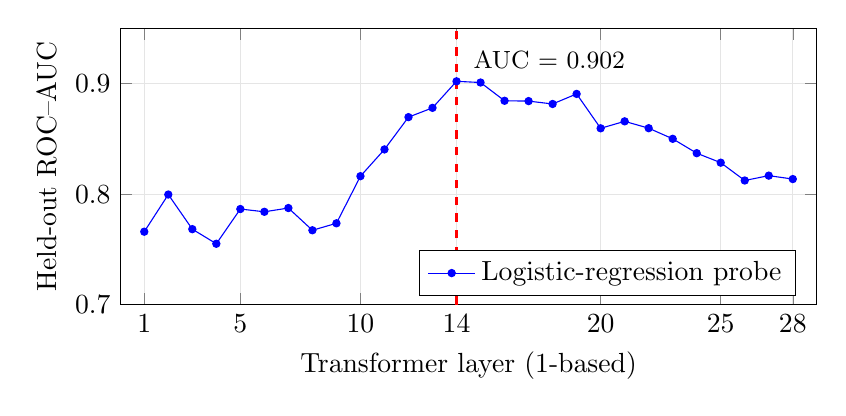
\begin{tikzpicture}
\begin{axis}[
  width=0.86\textwidth, height=0.42\textwidth,
  xlabel={Transformer layer (1-based)},
  ylabel={Held-out ROC--AUC},
  xmin=0, xmax=29, ymin=0.7, ymax=0.95,
  xtick={1,5,10,14,20,25,28},
  grid=both, grid style={gray!20},
  legend pos=south east, legend cell align=left,
]
\addplot[blue,mark=*,mark size=1.3pt] coordinates {
(1,0.766)(2,0.7996)(3,0.7683)(4,0.7551)(5,0.7865)(6,0.784)(7,0.7874)(8,0.7673)
(9,0.7736)(10,0.8162)(11,0.8404)(12,0.8696)(13,0.878)(14,0.902)(15,0.9009)
(16,0.8844)(17,0.8841)(18,0.8815)(19,0.8906)(20,0.8595)(21,0.8658)(22,0.8596)
(23,0.85)(24,0.837)(25,0.8284)(26,0.8123)(27,0.8167)(28,0.8136)
};
\addlegendentry{Logistic-regression probe}
\draw[red,dashed,thick] (axis cs:14,0.7) -- (axis cs:14,0.95);
\node[anchor=south west] at (axis cs:14.3,0.905) {\small AUC = 0.902};
\addlegendentry{}
\end{axis}
\end{tikzpicture}
\caption{Held-out ROC--AUC of a per-layer logistic-regression probe trained on last-token
hidden states of \texttt{Qwen2.5-1.5B-Instruct} for the TruthfulQA hallucination-detection
task. The strongest signal lies at layer 14 of 28 ($\sim$50\% depth), reproducing the
H-Node paper's prediction of a mid-network peak. The red dashed line marks $\ell^\star$.}
\label{fig:auc}
\end{figure}

\subsection{H-Node identification}
The top 50 H-Nodes (dimensions of $\mathbf{w}^{(14)}$ with the largest positive coefficients)
form a sparse set: of the 1536 hidden-state dimensions, only 50 ($\sim$3.3\%) carry the bulk
of the probe's signal. The first ten H-Node indices are
\[
\mathcal{H}_{1:10} = \{137,\ 357,\ 1102,\ 425,\ 1437,\ 450,\ 131,\ 1311,\ 686,\ 1054\}.
\]
Each dimension has an associated grounded baseline (the $80^{\text{th}}$ percentile of its
value among the grounded training prompts); the H-Node excess of a new prompt is the mean
clipped-positive excursion above these baselines.

\subsection{Live detection on novel prompts}
Table~\ref{tab:detect} reports the \texttt{detect} stage on six probe-naive prompts spanning
common factual question--answer pairs. Four of the six are classified correctly, including
all four hallucinated cases. The two errors --- the grounded \texttt{"Paris"} and
\texttt{"4"} answers --- are discussed in Section~\ref{sec:fp}.

\begin{table}[h]
\centering
\caption{Live detection on 6 demo prompts. Threshold $=0.5$.}
\label{tab:detect}
\begin{tabular}{llllr}
\toprule
\textbf{Prompt} & \textbf{Expected} & \textbf{Verdict} & $P(\text{hall})$ & \textbf{H-excess}\\
\midrule
\texttt{Q: capital of France?\ \ A: Paris}        & grounded     & hall.\ $\times$   & 1.000 & 0.211\\
\texttt{Q: capital of France?\ \ A: London}       & hallucinated & hall.\ \checkmark & 1.000 & 0.345\\
\texttt{Q: Who wrote Hamlet?\ \ A: Shakespeare}   & grounded     & ground.\ \checkmark & 0.002 & 0.205\\
\texttt{Q: Who wrote Hamlet?\ \ A: Charles Dickens} & hallucinated & hall.\ \checkmark & 1.000 & 0.271\\
\texttt{Q: What is 2 + 2?\ \ A: 4}                & grounded     & hall.\ $\times$   & 1.000 & 0.307\\
\texttt{Q: What is 2 + 2?\ \ A: 5}                & hallucinated & hall.\ \checkmark & 1.000 & 0.337\\
\midrule
\textbf{Accuracy on demo set} & & & & \textbf{4/6 (66.7\%)}\\
\bottomrule
\end{tabular}
\end{table}

The predicted probabilities are highly decisive (correct grounded answers near $0.00$,
everything classified hallucinated at $\approx 1.00$): the probe behaves as a high-confidence
classifier on this out-of-distribution demo set, which both helps (sharp margins on the true
hallucinations) and hurts (saturated false positives, Section~\ref{sec:fp}).

% ===========================================================================
\section{Discussion}

\subsection{What worked}
\begin{enumerate}
  \item \textbf{The detection use case survives the rewrite.} No modifications were required
  to the worker, the framework's hook installation logic, or vLLM itself --- only a new
  analyzer adapted to the \texttt{analyze(spec, run\_id, probes)} contract and registered
  through the standard plugin system. The migration is essentially mechanical once the new
  contracts are understood, and the upstream \texttt{ScienceHallucinationAnalyzer} serves as a
  faithful template.
  \item \textbf{The probe signal is real and structured.} A held-out AUC of 0.902 is well
  above chance, and the per-layer curve (Figure~\ref{fig:auc}) shows the predicted
  monotone build-up to a mid-network peak followed by decay, independently reproducing the
  H-Node paper's central claim on a different (smaller) model than the previous iteration.
  \item \textbf{End-to-end inference is fast and hardware-modest.} On the RTX 4060, detection
  adds essentially no latency over a vanilla vLLM forward pass, and the entire pipeline runs
  inside 8\,GB of VRAM with FlashAttention on vLLM's V1 engine --- no specialised hardware or
  attention-backend overrides, in contrast to the previous T4-era configuration.
\end{enumerate}

\subsection{The false positives}\label{sec:fp}
Two grounded prompts (\texttt{"Paris"} and \texttt{"4"}) are misclassified as hallucinated.
The \texttt{"Paris"} error mirrors the previous iteration and reflects a property of TruthfulQA
as a training distribution: TruthfulQA is deliberately built around \emph{common
misconceptions}, so its correct answers are typically counter-intuitive corrections of
widely-held false beliefs. The probe therefore learns the implicit rule
\emph{``high-confidence common-knowledge factoid $\Rightarrow$ likely a misconception
$\Rightarrow$ probably wrong''}, which generalises poorly to neutral common-knowledge
questions. The additional \texttt{"4"} false positive (absent in the previous 3B run) is
attributable to the smaller 1.5B model and its more saturated probe: the held-out AUC here
(0.902) is below the 3B's (0.919), and the demo-set accuracy correspondingly drops from 5/6 to
4/6. Both errors are distributional, not algorithmic; broadening the grounded class with
neutral common-knowledge QA (TriviaQA, NaturalQuestions) and/or using a larger backbone would
break the spurious correlation.

\subsection{Limitations}
\begin{itemize}
  \item \textbf{Model size forced by VRAM.} The 8\,GB budget required dropping from
  \texttt{Qwen2.5-3B} to \texttt{Qwen2.5-1.5B}. The smaller model yields a weaker, more
  overconfident probe (lower held-out AUC, more demo false positives). The pipeline is
  model-agnostic; only the \texttt{model\_configs/...} JSON files are model-specific.
  \item \textbf{Small training set.} 600 prompts suffice to fit a linear probe on a
  1536-dimensional space without catastrophic overfitting, but cap achievable generalisation.
  \item \textbf{Linear, inference-only probe.} We implement Phase~1 only; nonlinear probes
  might extract a stronger signal at the cost of H-Node interpretability, and the attack /
  defense phases are not implemented.
  \item \textbf{Pinned, slightly fragile environment.} The working stack depends on specific
  pins (\texttt{vllm==0.11.0}, \texttt{transformers==4.57.1}) and a \texttt{\_bz2} shim around
  a mis-built system Python; a clean Python 3.11/3.12 build would remove the shim.
\end{itemize}

% ===========================================================================
\section{Conclusion and Future Work}

This project confirms that the H-Node detection use case ports cleanly onto the current
vLLM-Hook framework: the detector is re-expressed entirely within the new plugin contracts,
with no changes to the framework core, and continues to produce a usable signal. A
logistic-regression probe trained on 420 TruthfulQA prompts at layer~14 of
\texttt{Qwen2.5-1.5B-Instruct} achieves held-out ROC--AUC 0.902, and end-to-end live detection
on the RTX~4060 produces 4/6 correct verdicts on a probe-naive demo set with sharp probability
margins. Beyond the empirical demonstration, the rebased repository contributes: (i) a
model-agnostic \texttt{hallucination\_detection/} package; (ii) a \texttt{HallucinationAnalyzer}
adapted to the post-refactor analyzer contract and integrated into the existing registry;
(iii) a three-stage CLI driver and reusable model configurations for the 1.5B and 3B models.

\subsection{Future work}\label{sec:future}
\begin{enumerate}
  \item \textbf{Larger backbone on more VRAM.} Repeat on \texttt{Qwen2.5-3B}/\texttt{7B} on a
  $\ge 16$\,GB GPU to recover the stronger 3B-era signal and reduce false positives.
  \item \textbf{Broader training distribution.} Augment TruthfulQA with TriviaQA and
  NaturalQuestions to remove the misconception-class bias responsible for the \texttt{"Paris"}
  false positive.
  \item \textbf{H-Node defense (Phase~3).} Add a steering worker that writes corrections back
  into the residual stream at $\ell^\star$ when the H-Node excess exceeds a threshold. The new
  framework's \texttt{SteerHookActWorker} and \texttt{extra\_args} steering hook make this a
  well-scoped extension.
  \item \textbf{Serve-path detection.} Re-validate through \texttt{HookClient} against a
  running \texttt{vllm serve} endpoint, exercising the \texttt{vllm\_xargs} transport.
  \item \textbf{Threshold calibration.} Replace the conventional $0.5$ threshold with an
  operating point chosen from a precision--recall curve on a labelled production-traffic
  sample.
\end{enumerate}

% ===========================================================================
\section*{Acknowledgements}
The vLLM-Hook framework was developed by IBM Research and made available as the starting
artefact for this project; the upstream \texttt{ScienceHallucinationAnalyzer} and
\texttt{demo\_scihal.py} served as the reference template for the post-refactor analyzer
contract. The H-Node Adversarial Neural Computation framework is due to Yocam, Vaidyan, and
Wang (2026). All implementation, migration, experimentation, and analysis reported herein are
the author's own work.

% ===========================================================================
\begin{thebibliography}{9}
\bibitem{vllm} W. Kwon, Z. Li, S. Zhuang, Y. Sheng, L. Zheng, C. H. Yu, J. Gonzalez,
H. Zhang, and I. Stoica, \emph{Efficient Memory Management for Large Language Model Serving
with PagedAttention}, SOSP, 2023.
\bibitem{hnode} E. Yocam, M. Vaidyan, and L. Wang, \emph{H-Node Attack and Defense in Large
Language Models}, 2026 (manuscript).
\bibitem{truthfulqa} S. Lin, J. Hilton, and O. Evans, \emph{TruthfulQA: Measuring How Models
Mimic Human Falsehoods}, ACL, 2022.
\bibitem{triviaqa} M. Joshi, E. Choi, D. S. Weld, and L. Zettlemoyer, \emph{TriviaQA: A Large
Scale Distantly Supervised Challenge Dataset for Reading Comprehension}, ACL, 2017.
\bibitem{nq} T. Kwiatkowski, J. Palomaki, O. Redfield, M. Collins, A. Parikh, et al.,
\emph{Natural Questions: A Benchmark for Question Answering Research}, TACL, vol.~7, 2019.
\end{thebibliography}

% ===========================================================================
\appendix
\section{Reproducibility}

\subsection{Repository}
The rebased code is available at the author's GitHub fork:
\begin{center}
\url{https://github.com/Samarpit-bhatia/vLLM-Hook}
\end{center}
Upstream framework: \url{https://github.com/IBM/vLLM-Hook}. The feature is re-applied as a
single commit on top of the latest upstream; the pre-rebase history is preserved on a local
\texttt{pre-rebase-backup} branch.

\subsection{One-shot reproduction}
On a Linux machine with an NVIDIA GPU of compute capability $\ge 8.0$:
\begin{lstlisting}[style=sh]
# 1. Create venv and install the pinned stack.
#    NOTE: point TMPDIR at a large partition -- pip unpacks wheels in /tmp,
#    which may sit on a small root partition.
python3 -m venv .venv
.venv/bin/pip install --upgrade pip
TMPDIR=$PWD/.pip-tmp .venv/bin/pip install --no-cache-dir \
    "vllm==0.11.0" "transformers==4.57.1" scikit-learn datasets

# 2. Editable-install the plugin package (registers the entry points).
TMPDIR=$PWD/.pip-tmp .venv/bin/pip install --no-cache-dir -e vllm_hook_plugins

# (Only if the Python build lacks _bz2: add a shim so transformers imports.)
#   see report Section 4.6, item 4.

# 3. Run the three stages (keep temp/cache off the small root partition).
export TMPDIR=$PWD/.localtmp VLLM_CACHE_ROOT=$PWD/.localtmp/vllm_cache \
       HF_HOME=$PWD/cache/hf
.venv/bin/python examples/demo_halludetect.py extract
.venv/bin/python examples/demo_halludetect.py train
.venv/bin/python examples/demo_halludetect.py detect
\end{lstlisting}

\subsection{Key result artefacts}
\begin{itemize}
  \item \texttt{hallucination\_detection/artifacts/activations.pt} --- 103\,MB,
  $600 \times 28 \times 1536$ fp32 last-token activations + labels + question IDs.
  \item \texttt{hallucination\_detection/artifacts/probe.npz} + \texttt{probe.json} ---
  best layer 14, AUC 0.902, 50 H-Nodes, per-layer AUC dictionary.
\end{itemize}

\end{document}
